\chapter{Evaluation}
\label{chp:ch7-evaluation}

To fully evaluate the effectiveness of the optimizations we discussed in the Chapter~\ref{chp:ch4-zippy}, Chapter~\ref{chp:ch5-peeling} and Chapter~\ref{chp:ch6-object}, we evaluate the performance of ZipPy in the following steps:
First we evaluate the overall performance of ZipPy by running a selection of conventional benchmarks.
These benchmarks are popular among the virtual machine research and Python communities.
They provide a good indication of the overall performance of a programming language implementation.
Second we examine the effectiveness of generator peeling using a set of real world and generator intensive Python programs.
As the last step, we analyze the performance and space impact of using flexible object storage generation in ZipPy.
We organize our extensive performance experiments by comparing ZipPy with the existing Python VMs.

\section{The Performance of ZipPy}
\label{sec:ch6-performance-of-zippy}

\subsection{Experiment Setup}

We evaluate the overall performance of ZipPy by comparing the performance of our system with existing Python VMs, such as CPython~\cite{python}, Jython~\cite{jython} and PyPy~\cite{pypy}.
Our system setup is as follows:

\begin{itemize}

\item Intel Xeon E5462 Quad-Core processor running at a frequency of 2.8GHz, on Mac OS X version 10.9.3 build 13D65.

\item Apple LLVM 5.1, OpenJDK 1.8.0\_05, Truffle/Graal 0.3.\footnote{From source code repository \url{http://hg.openjdk.java.net/graal/graal}}

\end{itemize}

The VM versions used in the comparison and the description of their execution models are as follows:

\begin{itemize}

\item CPython 2.7.6 and 3.4.0: Interpreter only.

\item Jython 2.7-beta2:
Python 2 compliant, hosted on JVMs.
Compiles Python modules to Java classes and lets the JVM JIT compiler further compiles them to machine code.

\item PyPy 2.3.1 and PyPy3 2.3.1: Python 2 and 3 compliant respectively.
Uses a meta-tracing JIT compiler that compiles Python code to machine code.

\end{itemize}

% Python 2 vs. Python 3
Python 3 is not backward compatible with Python 2.
Although ZipPy exclusively supports Python 3, including well-established Python 2 VMs in the comparison highlights the potential of our optimization.
The benchmarks we chose support both Python 2 and 3.
The same code, however, suffers from a slight difference in the semantics interpreted by different VMs.

% how we measure, peak performance
We run each benchmark ten times on each VM and average the execution times.
For VMs that use a tiered execution strategy, we warm up the benchmarks to ensure that the code is just-in-time compiled.
This allows us to properly measure peak performance.

\subsection{Benchmark Selection}

\begin{table*}
  \begin{center}
    \begin{tabular}{ l l }
    \toprule
    Benchmark suite & Included benchmarks \\
    \midrule
	Computer Language Benchmarks - & \textsf{binarytrees}, \textsf{fannkuchredux}, \textsf{fasta}, \textsf{mandelbrot}, \textsf{meteor} \\
	Games & \textsf{nbody}, \textsf{pidigits}, \textsf{spectralnorm} \\
	\midrule
	Unladen Swallow Benchmarks &  \textsf{float}, \textsf{richards} \\
	\midrule
	PyPy Benchmarks & \textsf{chaos}, \textsf{deltablue}, \textsf{go} \\
    \bottomrule
	\end{tabular}
    \caption{Benchmarks selection}
    \label{tab:ch6-regular-benchmark-selection}
  \end{center}
\end{table*}

We selected a number of benchmarks for the performance experiments from three popular benchmark suites.
The descriptions of the chosen benchmark suites are as follows:

\begin{itemize}

\item Computer Language Benchmarks Game~\cite{benchmarkgame}: a popular benchmark suite for evaluating and comparing the performance of different programming languages.

\item Unladen Swallow Benchmarks~\cite{unladen.swallow}: the benchmark suite used by the unladen swallow project.
Unladen swallow is an optimization branch of CPython built by Google.
The goal of the project was to become a faster yet fully compatible modification of CPython.
Its benchmark suite is well-regarded in the Python community.

\item PyPy Benchmarks: a collection of benchmarks used by the PyPy project.

\end{itemize}

Table~\ref{tab:ch6-regular-benchmark-selection} summarizes the benchmarks we selected in this experiment from the above mentioned suites.
Since we focus on the overall performance of Python VMs, we intentionally leave out benchmarks that are sensitive to the performance of generators.
We selected benchmarks that are written in both imperative and object oriented styles.

\subsection{Experiment Results}

\begin{table*}
  \small
  \begin{center}
  \begin{tabular}{ l r r r r r r }
  \toprule
  Benchmark     & CPython3  & CPython  & Jython  & PyPy     & PyPy3    & ZipPy \\
  \midrule
  \textsf{binarytrees}   & $5.40$    & $5.10$   & $10.76$ & $14.05$  & $14.60$  & $39.49$ \\
  \textsf{fannkuchredux} & $2.27$    & $2.20$   & $1.17$  & $101.24$ & $107.52$ & $198.94$ \\
  \textsf{fasta}         & $15.52$   & $16.20$  & $24.13$ & $182.09$ & $174.55$ & $241.76$ \\
  \textsf{mandelbrot}    & $9.00$    & $9.70$   & $3.03$  & $98.15$  & $97.35$  & $105.18$ \\
  \textsf{meteor}        & $100.55$  & $102.83$ & $77.14$ & $265.43$ & $263.75$ & $213.77$ \\
  \textsf{nbody}         & $10.12$   & $9.87$   & $7.40$  & $122.83$ & $122.07$ & $62.42$ \\
  \textsf{pidigits}      & $77.02$   & $77.40$  & $47.59$ & $75.25$  & $73.02$  & $46.59$ \\
  \textsf{spectralnorm}  & $0.90$    & $1.20$   & $1.70$  & $114.60$ & $114.52$ & $115.29$ \\
  \textsf{float}         & $10.82$   & $10.23$  & $11.37$ & $93.57$  & $93.82$  & $191.68$ \\
  \textsf{richards}      & $16.77$   & $15.83$  & $20.35$ & $495.38$ & $490.70$ & $840.93$ \\
  \textsf{chaos}         & $2.05$    & $2.40$   & $3.17$  & $83.77$  & $52.65$  & $139.94$ \\
  \textsf{deltablue}     & $19.62$   & $16.77$  & $26.19$ & $590.25$ & $571.82$ & $460.37$ \\
  \textsf{go}            & $23.15$   & $24.97$  & $46.16$ & $157.29$ & $154.07$ & $356.80$ \\
  \bottomrule
  \end{tabular}
  \caption{The scores of Python VMs running regular benchmarks}
  \label{tab:ch6-regular-benchmarks-scores}
  \end{center}
\end{table*}

\begin{table*}
  \small
  \begin{center}
  \begin{tabular}{ l r r r r r r }
  \toprule
  Benchmark     & CPython3  & CPython  & Jython  & PyPy     & PyPy3    & ZipPy \\
  \midrule
  \textsf{binarytrees}   & $1.00$    & $0.94$   & $1.99$  & $2.60$   & $2.70$   & $7.31$ \\
  \textsf{fannkuchredux} & $1.00$    & $0.97$   & $0.51$  & $44.53$  & $47.29$  & $87.50$ \\
  \textsf{fasta}         & $1.00$    & $1.04$   & $1.55$  & $11.73$  & $11.24$  & $15.57$ \\
  \textsf{mandelbrot}    & $1.00$    & $1.08$   & $0.34$  & $10.91$  & $10.82$  & $11.69$ \\
  \textsf{meteor}        & $1.00$    & $1.02$   & $0.77$  & $2.64$   & $2.62$   & $2.13$ \\
  \textsf{nbody}         & $1.00$    & $0.97$   & $0.73$  & $12.13$  & $12.06$  & $6.17$ \\
  \textsf{pidigits}      & $1.00$    & $1.00$   & $0.62$  & $0.98$   & $0.95$   & $0.60$ \\
  \textsf{spectralnorm}  & $1.00$    & $1.33$   & $1.89$  & $127.33$ & $127.25$ & $128.10$ \\
  \textsf{float}         & $1.00$    & $0.95$   & $1.05$  & $8.64$   & $8.67$   & $17.71$ \\
  \textsf{richards}      & $1.00$    & $0.94$   & $1.21$  & $29.53$  & $29.25$  & $50.13$ \\
  \textsf{chaos}         & $1.00$    & $1.17$   & $1.55$  & $40.88$  & $25.69$  & $68.28$ \\
  \textsf{deltablue}     & $1.00$    & $0.85$   & $1.33$  & $30.08$  & $29.14$  & $23.46$ \\
  \textsf{go}            & $1.00$    & $1.08$   & $1.99$  & $6.79$   & $6.66$   & $15.41$ \\
  \textbf{mean}          & \textbf{1.00}    & \textbf{1.02}   & \textbf{1.05}  & \textbf{12.15}  & \textbf{11.68}  & \textbf{15.34} \\
  \bottomrule
  \end{tabular}
  \caption{The speedups of Python VMs normalized to CPython3 running regular benchmarks}
  \label{tab:ch6-regular-benchmarks-speedups}
  \end{center}
\end{table*}

Table~\ref{tab:ch6-regular-benchmarks-scores} and~\ref{tab:ch6-regular-benchmarks-speedups} shows the results of our experiments.
We use a score system to gauge VM performance.
We calculate the score by dividing $1000$ by the execution time of the benchmark.
A score system is more intuitive than execution times for visualization purpose.
It also offers a higher resolution for our performance measurements.
We carefully chose the program inputs such that the resulting scores stay in the range between $10$ and $1000$.
Larger inputs have limited impacts on the speedups our of optimization.

Table~\ref{tab:ch6-regular-benchmarks-scores} shows the average scores of each Python VM running the selected benchmarks.
Table~\ref{tab:ch6-regular-benchmarks-speedups} shows the average speedups of each VM against CPython3.
We calculate the speedups by normalizing the scores of each VM shown in Table~\ref{tab:ch6-regular-benchmarks-scores} against that of CPython3.
The last row of Table~\ref{tab:ch6-regular-benchmarks-speedups} shows the geometric mean of the speedups of each Python VM relative to CPython3.
As shown in the Table, the average speedup of ZipPy over CPython3 is $\zippyToCPythonRegular{}\times$ with the highest speedup over $128\times$ on \textsf{spectralnorm}.
Note that the performance of ZipPy running the selected benchmarks is even higher than PyPy by around $26\%$

\subsection{Performance Analysis}

The majority of the high number speedups of ZipPy comes from compute intensive benchmarks like the ones from the Computer Language Benchmarks Game.
The unboxed data representation of numeric types in ZipPy successfully optimizes these benchmarks without ever having to go to the boxed representation.
At peak performance, ZipPy executes the entire benchmark by only using Java primitives for arithmetic operations.
This approach effectively enables low level optimizations offered by the underlying Graal compiler, which consequently achieved Java like arithmetics performance for Python programs in our experiments.
Being able to speculatively bring the cost of arithmetic operations in Python much closer to the one in Java is the key distinguisher between ZipPy and the existing JVM-based Python implementations.

The noticeable slow down in \textsf{pidigits} is caused by integer overflows in Python.
After an integer overflow, ZipPy uses a JDK \texttt{BigInteger}~\cite{hotspot} to model integers of a large value.
However, the implementation of \texttt{BigInteger} in the JDK did not outperform the implementation of \texttt{PyInt} in CPython on our benchmark.
We did not pursue in the direction of replacing \texttt{BigInteger} with a more efficient alternative written in Java, since we consider the implementation details of an unbound integer type to be orthogonal to the research we discuss in this thesis.

We also see speedups of multiple of $10\times$ on object-bound benchmarks like \textsf{richards} and \textsf{chaos}.
We only use fixed object storages in this experiment.
The results suggest that the Python object model used in ZipPy is orders of magnitude more efficient that the hash map based ones used in CPython and Jython.
The object layout based approach in ZipPy clears the way on letting the underlying Java compiler to optimize Python object accesses the same way as it does to Java objects.
In the common case where the object layouts stabilize shortly after warming up, ZipPy essentially delivers Java like performance on Python object operations in our experiment.

Overall ZipPy outperforms PyPy in our experiment.
We attribute this advancement to Graal, the underlying Java JIT compiler.
PyPy uses a relatively straight forward tracing JIT compiler to compile Python programs down to machine code.
Whereas Graal is a substantially more sophisticated and aggressive method JIT.
The kinds of optimizations implemented in Graal outnumbered that in PyPy.
Overall we do expect Graal to generate more efficient machine code that the compiler in PyPy.

In general the speedups we achieved in our experiment are inline with other efficient Truffle language implementations~\cite{seaton2014debugging,Grimmer+2014,Grimmer+2014TruffleC}.
A number of semi built-in optimizations offered by Truffle helped us achieving this result.
The most important ones includes: frame optimization that eliminates the heap allocation of a frame object and Truffle AST inlining.
Another advantage of using Truffle as the base of ZipPy is that it makes it easy for guest language implementers to fine tune the machine code size produced by the compiler.
It offers utilities that helps us to precisely specify the boundary of a JIT compilation rather than fully relying on the compiler heuristics.
This features allows us to carve out less important code paths from the compiled code to make the machine code size more compact.
In summary, by making better use of Truffle ZipPy is able to achieve high speedups when compared with existing Python VMs with low implementation cost.

\section{The Effectiveness of Generator Peeling}

We evaluate the performance of our generator peeling implementation in ZipPy by running Python programs that have intense use of generators.
We used the same experiment setup as we did in the overall performance evaluation of ZipPy in Section~\ref{sec:ch6-performance-of-zippy}.

\subsection{Benchmark Selection}

% benchmark selection
We analyzed hundreds of programs listed on the Python Package Index~\cite{pypi}.
We picked a set of programs that includes compute intensive benchmarks as well as larger applications.
The following chosen programs use generators to various degrees:

\begin{itemize}

\item \textsf{nqueens} is a brute force N-queens solver selected from the Unladen Swallow benchmark suite~\cite{unladen.swallow}.

\item The publicly available solutions to the first $50$ Project Euler problems~\cite{projecteuler}:
\textsf{euler11} computes the greatest product of four adjacent numbers in the same direction in a matrix;
\textsf{euler31} calculates the combinations of English currency denominations.

\item Python Algorithms and Data Structures (PADS) library~\cite{pads}:
\textsf{eratos} implements a space-efficient version of sieve of Eratosthenes;
\textsf{lyndon} generates Lyndon words over an s-symbol alphabet;
\textsf{partitions} performs integer partitions in reverse lexicographic order.

\item \textsf{pymaging} is a pure Python imaging library.
The benchmark draws a number of geometric shapes on a canvas.

\item \textsf{python-graph} is a pure Python graph library.
The benchmark processes a deep graph.

\item \textsf{simplejson} is a simple, fast JSON library.
The benchmark encodes Python data structures into JSON strings.

\item \textsf{sympy} is a Python library for symbolic mathematics.
The benchmark performs generic unifications on expression trees.

\item \textsf{whoosh} is a text indexing and searching library.
The benchmark performs a sequence of matching operations.

\end{itemize}

We learned from our generator survey that popular HTML template engines written in Python use generators.
There are two reasons we do not include them in our performance evaluation.
First, we implement ZipPy from scratch.
It is infeasible for us to support all Python standard libraries required to run these applications.
Second, many of these applications are not compute intensive.
They spent most of the execution time processing Unicode strings or in native libraries, which is not a good indicator of the VM performance.

\subsection{Experiment Results}

\begin{table*}
  \begin{center}
    \begin{tabular}{ l r r r r r r }
      \toprule
      Benchmark             & Score $-$GP & Score $+$GP & Speedup        & No. gen & No. genexp & No. of lines \\
      \midrule
      \textsf{nqueens}      &  $69.09$    & $313.14$    & \textbf{4.53}  & 2/2 & 5/5 & $41$ \\
      \textsf{euler11}      &  $71.42$    & $941.73$    & \textbf{13.19} & 2/2 & 5/5 & $61$ \\
      \textsf{euler31}      &  $47.70$    & $134.35$    & \textbf{2.82}  & 1/1\textsuperscript{\textdagger} & 2/2 & $46$ \\
      \textsf{eratos}       &  $277.13$   & $316.64$    & \textbf{1.14}  & 2/2 & 0/0 & $86$ \\
      \textsf{lyndon}       &  $37.89$    & $859.91$    & \textbf{22.69} & 3/3 & 0/0 & $127$ \\
      \textsf{partitions}   &  $50.36$    & $217.56$    & \textbf{4.32}  & 1/1 & 0/0 & $228$ \\
      \textsf{pymaging}     &  $102.80$   & $283.99$    & \textbf{2.76}  & 2/2 & 0/0 & $1528$ \\
      \textsf{python-graph} &  $51.89$    & $93.08$     & \textbf{1.79}  & 2/2 & 2/2 & $3136$ \\
      \textsf{simplejson}   &  $66.12$    & $242.52$    & \textbf{3.67}  & 1/1 & 0/0 & $3128$ \\
      \textsf{sympy}        &  $198.55$   & $259.68$    & \textbf{1.31}  & 4/5\textsuperscript{\textdagger} & 1/2 & $262k$ \\
      \textsf{whoosh}       &  $242.74$   & $676.10$    & \textbf{2.79}  & 4/4 & 0/0 & $40k$ \\
      \textbf{mean}         &             &             & \textbf{3.58}  &     &     & \\
      \bottomrule
	\end{tabular}
    \begin{tablenotes}
    \item \textsuperscript{\textdagger} Contains recursive generator calls.
    \end{tablenotes}
    \caption{The performance numbers of generator peeling}
    \label{tab:ch6-peeling-benchmark-scores}
  \end{center}
\end{table*}

Table~\ref{tab:ch6-peeling-benchmark-scores} shows the results of our experiments.
We use a score system to gauge VM performance.
We calculate the score by dividing $1000$ by the execution time of the benchmark.
A score system is more intuitive than execution times for visualization purpose.
It also offers a higher resolution for our performance measurements.
We carefully chose the program inputs such that the resulting scores stay in the range between $10$ and $1000$.
Larger inputs have limited impacts on the speedups our of optimization.

The second and third rows of Table~\ref{tab:ch6-peeling-benchmark-scores} show the score of each benchmark without and with the generator peeling optimization respectively.
The speedup row gives the speedups of our optimization.
The geometric mean of the speedups is $\peelingSpeedup{}\times$.
The following two rows of Table~\ref{tab:ch6-peeling-benchmark-scores} show the number of generator loops and generator expressions (implicit generator loops) used in the benchmarks as well as how many of them are successfully optimized using generator peeling.
The number on the left in each cell is the number of optimized generator loops, and the number on the right is the total number generator loops used in the benchmark.
Note that we only count generator loops that are executed by the benchmarks, since these are the ones that we can potentially optimize.
Table~\ref{tab:ch6-peeling-benchmark-scores} also shows, for each benchmark, the number of lines of Python code in the bottom row.

\subsection{Performance Analysis}

Our experiments show that generator peeling covers most instances of generator loops used in the benchmarks and results in speedups of up to an order of magnitude.
The following four steps explain how we obtain this performance.

\begin{enumerate}
\item Generator peeling eliminates the allocation of generator objects.
\item Generator peeling eliminates expensive suspend and resume control-flow transfers and replaces them with local variable assignments.
\item The optimized generator loops avoid the use of generator ASTs, which enables frame optimizations provided by the underlying JIT compiler.
The implicit generator loop transformation eliminates the closure behavior of the generator expressions and enables frame optimization of the enclosing scope.

% bigger context for compiler optimizations.
\item Generator peeling increases the scope of optimizations for the underlying compiler.
As a result, generator peeling creates more optimization opportunities for the compiler, resulting in better optimized code.
\end{enumerate}

To verify that generator peeling completely eliminates the overhead incurred by generators, we rewrote the benchmark \textsf{nqueens} to a version that only uses loops instead of generators.
We compare the scores of ZipPy running the modified version and the original benchmark with generator peeling enabled.
We found that generator peeling delivers the same performance on the original benchmark as manually rewriting generator functions to loops.

\begin{figure}
\centering
\includegraphics[scale=.58, page=2]{benchmarks/generator-peeling-benchmark-chart}
\caption{Detailed speedups of different Python implementations normalized to CPython 3.4.0}
\label{fig:ch6-generator-benchmark-zippy-speedup}
\end{figure}

However, the number of optimized generator loops does not directly relate to the speedups we observed.
The time each program spends in generator loops varies from one to another.
The shorter the time a program spends in generator loops, the smaller the speedup resulting from our optimization.
For each generator loop, the overhead-to-workload ratio is the overhead incurred by the generators divided by the actual computation performed in the loop.
Generator loops with a higher overhead-to-workload ratio achieve higher speedups from generator peeling.
Loops in which the actual computation dominates overall execution benefit less from generator peeling.

For instance, \textsf{euler11} is a compute intensive program where generator overhead dominates the execution.
Generator peeling transfers the program into nested loops that perform mostly arithmetic, which is an ideal optimization target for the JIT compiler.
On the other hand, larger programs like \textsf{python-graph} contain extensive use of user-defined objects and other heap-allocated data structures.
The overhead-to-workload ratio in such programs is relatively low.
Although having the same number of generator functions optimized, generator peeling results in different speedups in these two programs.

% talk about polymorphisms.
Despite the fact that larger Python programs exhibit a large number of type changes, generator loops tend to remain stable.
Programmers tend to write generator loops that consume generator objects produced by the same generator function.
In our experiments, We only found a few number of polymorphic generator loops, which, as described in Section~\ref{sec:ch4-polymorphic-and-deopt}, our optimization is able to handle.

When optimizing nested generator loops, ZipPy starts by peeling off the root layer in a non-generator caller.
If it successfully optimizes the first layer, ZipPy continues to peel off subsequent layers.
If this iterative process fails at one layer, ZipPy stops peeling.
The benchmark \textsf{euler31} and \textsf{sympy} include recursive generator functions that contain calls to itself.
Such a recursive generator function effectively contains infinite levels of generator loops.
In other words, the optimized generator body always contain a generator loop that calls the same generator function.
The fixed inlining budget only allows ZipPy to optimize the first few invocations of a recursive generator function to avoid code explosion.
Generator peeling has limited impact on the performance of a deep recursive call to such a generator function.
This incomplete coverage of recursive generator functions is an implementation limitation.

% discussion on the impact to the compilation time
Generator peeling is essentially a speculative AST level transformation that is independent from JIT compilation.
Not only does it improve peak performance, it also speeds up interpretation before the compilation starts.
Generator peeling does not introduce new optimization phases to the compiler, rather it simplifies the workload for the underlying compiler.
For the nested generator loops case, generator peeling does increase the AST size but it also reduces the number of functions that need to be compiled.
In general, generator peeling has negligible impact on the compilation times.

% ZipPy vs. PyPy
\subsection{ZipPy vs. PyPy}

\begin{figure}
\centering
\subfigure[A generator loop example]{
	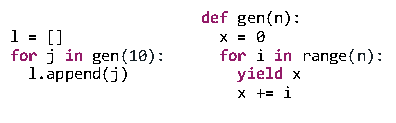
\includegraphics[scale=1.7]{figures/ch6-pypy-example-code}
	\label{fig:pypy_example_code}
}

\subfigure[Optimized trace of the generator loop example]{
	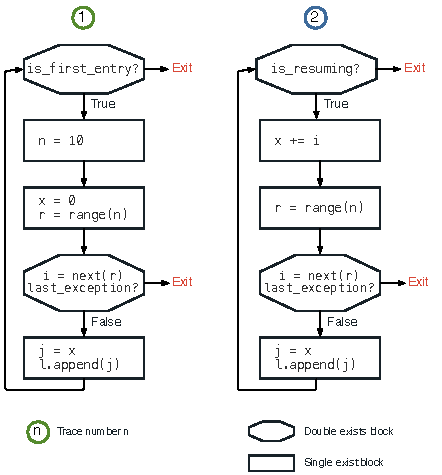
\includegraphics[scale=1.5]{figures/ch6-pypy-example-trace}
	\label{fig:pypy_example_trace}
}
\caption{Generator optimization in PyPy}
\label{fig:pypy_generator_inlining}
\end{figure}

PyPy is the state-of-the-art implementation of Python that implements a meta-tracing JIT compiler for aggressively optimizing Python programs~\cite{bolz.etal09,Rigo2006}.
PyPy is fairly mature and complete compared to ZipPy.

ZipPy on the other hand is more light weight in terms of implementation effort.
It benefits from low-cost speculative type specialization, which is the most critical performance optimization for dynamic languages.
ZipPy does not have to invest or maintain its own compilation infrastructure.
It relies on the underlying Java compiler to JIT compile Python code.
The Java JIT compiler is, in general, more sophisticated and aggressive than the one in PyPy.
Any additional optimizations added to Truffle will automatically benefit our system.

\subsubsection{PyPy's Generator Optimization}

\begin{table*}
  \begin{center}
  \begin{tabular}{ l r r }
  \toprule
  Benchmark             & Speedup $-$GP & Speedup $+$GP \\
  \midrule
  \textsf{nqueens}      & $0.52$ & $2.36$ \\
  \textsf{euler11}      & $0.72$ & $9.51$ \\
  \textsf{euler31}      & $0.60$ & $1.70$ \\
  \textsf{eratos}       & $2.30$ & $2.63$ \\
  \textsf{lyndon}       & $0.30$ & $6.71$ \\
  \textsf{partitions}   & $0.37$ & $1.58$ \\
  \textsf{pymaging}     & $0.55$ & $1.48$ \\
  \textsf{python-graph} & $0.51$ & $0.92$ \\
  \textsf{simplejson}   & $0.33$ & $1.22$ \\
  \textsf{sympy}        & $0.27$ & $0.36$ \\
  \textsf{whoosh}       & $0.90$ & $2.52$ \\
  \textbf{mean}         & \textbf{$0.55$} & \textbf{$1.95$} \\
  \bottomrule
  \end{tabular}
  \caption{The speedups of ZipPy without and with generator peeling normalized to PyPy3}
  \label{tab:ch6-generator-benchmarks-zippy-vs-pypy}
  \end{center}
\end{table*}

% PyPy inlining stuff
PyPy also supports a generator optimization that primarily targets simple generator functions in its recent releases.
Figure~\ref{fig:pypy_example_code} shows an example generator loop (left) that consumes a simple generator function (right).
We use this example to demonstrate PyPy's optimization.
PyPy is able to trace the execution of the loop and compiles it into machine code.
The trace compiler inlines the implicit call to the generator's \texttt{\_\_next\_\_} method into the loop body.
It does so by constant folding the \texttt{last\_instruction} pointer on the generator frame, which stores the suspended program location in the generator.
The subsequent compiler optimizations convert the \emph{yield} operation to a direct jump.
However, generator frame accesses are not fully optimized, since its allocation happens outside the trace and cannot be seen by the JIT compiler.

PyPy's trace compiler compiles linear execution paths into machine code.
Different iterations of a generator loop are likely to be compiled into different traces.
Figure~\ref{fig:pypy_example_trace} illustrates two different traces the compiler generates for our example.
We simplified the intermediate representation format in PyPy's trace to make it more readable.
The first iteration of the loop goes into trace one; the remaining iterations execute in trace two.
More complicated control structures and multiple yields in a generator function introduce more branches in the consuming loop.
The number of traces generated by the compiler increases for more complicated generators.
As a result, the execution of an optimized generator loop has to switch between different traces.
Not only does the trace switching incur slow paths, it also increases instruction cache misses.
Currently more complicated generators are not properly optimized by PyPy.

Generator peeling on the other hand is able to optimize more complicated generators.
ZipPy using the underlying method-based JIT compiler compiles the entire transformed generator loop into machine code, and completely removes overheads incurred by a generator.
Moreover, by analyzing the assembly code produced by both JIT compilers, we found that, even for a simple generator case, Truffle is able to produce more efficient machine code.
Table~\ref{tab:ch6-generator-benchmarks-zippy-vs-pypy} shows the speedups of ZipPy with and without generator peeling, relative to PyPy3 (Python 3).
The overall performance of ZipPy without generator peeling is competitive with PyPy3.
However, by enabling generator peeling, our system outperforms PyPy3 by a factor of two.

\section{The Effectiveness of Flexible Object Storages}

In the overall performance evaluation of ZipPy we used a fixed object storage configuration in our experiments.
Here we extend our experiments and evaluates the implementation of flexible object storage in ZipPy.
We do so by comparing the time and space efficiency between the different object model configurations in ZipPy.
We select a number of object-bound benchmarks from our comprehensive benchmark selection for this particular experiments.
Those benchmarks includes: \textsf{float}, \textsf{richards}, \textsf{chaos}, \textsf{deltablue} and \textsf{go}.
We used the same experiment setup as mentioned previously in Section~\ref{sec:ch6-performance-of-zippy}.

\subsection{Object Model Configurations}

As we discussed in Chapter~\ref{chp:ch6-object}, a fixed object storage has a fixed number of fields to stores Python object attributes.
To accommodate attributes modeled using Java primitive types, a fixed object storage needs to have fields of different types, such as Java \textsf{int}, \textsf{double} and \textsf{Object}.
In our experiment, we use fixed object storages that have equal number of fields of each of these three types.
Note that we cannot mix the fields of different types, since the binary representation of each type varies in different JVM implementations.
For instance, some versions of the HotSpot VM~\cite{hotspot} use a technique called pointer compression to reduce the size of a Java object pointer.
Therefore, storing a non-pointer value in a pointer field using \textsf{Unsafe} will lead to unexpected behavior at runtime.
The size of a fixed object storage refers to the number of fields of each type the storage has.
The bigger the storage size the more attribute it can accommodate in a field.
However, larger storage size also lead to memory space inefficiency.
Since a large portion of the object storage space maybe not be utilized.
In the overall performance evaluation, the space configuration of the fixed object storage used in ZipPy is five.

The size of a flexible object storage is determined at runtime.
The two different configurations we used in our experiment are \emph{simple flexible object storage} and \emph{flexible object storage with continuous generation}.
Simple flexible object storage means we only generate one storage class for each Python class.
We handle all post-constructor object layout change by using the spill array.
In flexible object storage with continuous generation, we always generate a new storage class whenever a layout change takes place.

\subsection{The Performance of Flexible Object Storages}

\begin{figure}
\centering
\includegraphics[scale=.4, page=4]{benchmarks/object-model-results}
\caption{Detailed speedups of different object model configurations normalized to fixed object storage of size $5$}
\label{fig:ch6-object-model-config-speedup}
\end{figure}

Figure~\ref{fig:ch6-object-model-config-speedup} shows the performance of each object model configuration running the selected benchmarks normalized to the fixed object storage.
With flexible object storage enabled we discover speedups when running the majority of the benchmarks with the highest speedup of $14\%$ on \textsf{chaos}.
The average speedup of using flexible object storage is $2$ to $3\%$.
We also notice a slowdown on \textsf{richards}.
The worse case slowdown caused by using flexible object storage is about $22\%$.

We did not observe more aggressive speedups, because of the high setting on the size of the baseline fixed object storage configuration.
A fixed object storage of size five has fifteen fields.
Given that most Python objects allocated at runtime are small in size, a fixed object storage of size five is in most cases more than enough to accommodate all the attributes of a Python object.
Having a high setting on the size of fixed object storage enables better performance but at the price of allocating more space for each Python object.

Flexible object storage on the other hand ensures that we allocate just enough memory space for a Python object.
Continuous storage class generation also guarantees that any new object allocation is performance wise optimal based on the latest layout description of the object.
On a few benchmarks enabling continuous storage class generation causes a moderate slowdown.
This slowdown is caused by higher degree of polymorphism potentially introduced by new storage class generation at an object access site.
After the generation of a new storage class, the Python object instances allocated using an old storage class might still be alive.
The mix of storage classes causes the access of Python objects of the same Python class to use multiple inline cache entries.
The increase in the number of cache entries leads to a slowdown that we observed in our results.
The more noticeable slowdown on \textsf{richards} when enabling flexible object storage is due to the current implementation of Truffle we used in this experiment.
Switching the object storage configuration causes a change in the AST inlining pattern for \textsf{richards}.
As a consequence, this pattern change results in a slowdown in our experiment.
We expect that using a newer version of Truffle with updated inlining heuristics will correct this fluctuation.

A fixed object storage configuration is always biased.
A single size configuration cannot work well for all Python programs let alone the fixed type distribute among the fields of an object storage.
Even with a high size setting, using fixed object storage is $14\%$ slower than the flexible approach as shown in Figure~\ref{fig:ch6-object-model-config-speedup}.
The reason behind is the allocation of large Python objects.
Any attribute that cannot fit into the fixed object storage is stored in the spill array.
The additional memory access incurred by accessing the spill array causes a slowdown on the benchmark.

\subsection{The Space Efficiency of Flexible Object Storages}

\begin{figure}
\centering
\includegraphics[scale=.45, page=5]{benchmarks/object-model-results}
\caption{The memory overheads of fixed object storage of size $1$, $3$ and $5$ relative to flexible storage allocation with continuous generation}
\label{fig:ch6-fixed-object-storage-space-overhead}
\end{figure}

\begin{figure}
\centering
\includegraphics[scale=.45, page=6]{benchmarks/object-model-results}
\caption{The slowdowns of fixed object storage of size $1$, $3$ and $5$ relative to flexible storage allocation with continuous generation}
\label{fig:ch6-fixed-object-storage-slowdown}
\end{figure}

We measured the memory space used to allocate fixed object storages for each selected benchmark with three distinct size settings: one, three and five.
We compare the memory space numbers with the equivalent measured using flexible object storage with continuous generation enabled.
Figure~\ref{fig:ch6-fixed-object-storage-space-overhead} shows the results of this experiment normalized to the memory space usage of flexible object storage.
Using a fixed object storage of size one allocates on average $1.63\times$ more memory than using flexible object storage.
Using a fixed object storage of size five allocates up to $3.6\times$ more memory than using the flexible configuration.

The result shows that using a fixed object storage causes a significant memory overhead.
We attribute this inefficiency to the poor type distribution among the fields of a fixed object layout.
In theory one could design an improved solution that generates a library of fixed object storage with various combination of sizes and type distributions ahead of time, and pick the closest fit from the library when allocating a Python object.
This hypothetical solution, even in an ideal case, cannot surpass flexible object storage in terms of space efficiency.
Since flexible object storage ensures the optimal space and type distribution allocated for a given Python object.

We also measured the slowdown of using a fixed object storage running the benchmarks compared to using flexible object storages.
The fixed object storage configurations used in our experiment includes the following size settings: one, three and five.
Figure~\ref{fig:ch6-fixed-object-storage-slowdown} shows the slowdowns of using various fixed object storages.
Overall we observe slowdowns ranging from $2$ to $20\%$ in the results.
The smaller the fixed object storage size the higher the slowdown.
Using a fixed object storage of size one causes a slowdown up to $20\%$ on \textsf{chaos}.
By increase the size of fixed object storages the slowdowns tend to decrease or even diminish.

%\fxnote{adding a discussion subsection?}
